% Options for packages loaded elsewhere
% Options for packages loaded elsewhere
\PassOptionsToPackage{unicode}{hyperref}
\PassOptionsToPackage{hyphens}{url}
\PassOptionsToPackage{dvipsnames,svgnames,x11names}{xcolor}
%
\documentclass[
  authoryear,
  doubleblind]{elsarticle}
\usepackage{xcolor}
\usepackage{amsmath,amssymb}
\setcounter{secnumdepth}{5}
\usepackage{iftex}
\ifPDFTeX
  \usepackage[T1]{fontenc}
  \usepackage[utf8]{inputenc}
  \usepackage{textcomp} % provide euro and other symbols
\else % if luatex or xetex
  \usepackage{unicode-math} % this also loads fontspec
  \defaultfontfeatures{Scale=MatchLowercase}
  \defaultfontfeatures[\rmfamily]{Ligatures=TeX,Scale=1}
\fi
\usepackage{lmodern}
\ifPDFTeX\else
  % xetex/luatex font selection
\fi
% Use upquote if available, for straight quotes in verbatim environments
\IfFileExists{upquote.sty}{\usepackage{upquote}}{}
\IfFileExists{microtype.sty}{% use microtype if available
  \usepackage[]{microtype}
  \UseMicrotypeSet[protrusion]{basicmath} % disable protrusion for tt fonts
}{}
\makeatletter
\@ifundefined{KOMAClassName}{% if non-KOMA class
  \IfFileExists{parskip.sty}{%
    \usepackage{parskip}
  }{% else
    \setlength{\parindent}{0pt}
    \setlength{\parskip}{6pt plus 2pt minus 1pt}}
}{% if KOMA class
  \KOMAoptions{parskip=half}}
\makeatother
% Make \paragraph and \subparagraph free-standing
\makeatletter
\ifx\paragraph\undefined\else
  \let\oldparagraph\paragraph
  \renewcommand{\paragraph}{
    \@ifstar
      \xxxParagraphStar
      \xxxParagraphNoStar
  }
  \newcommand{\xxxParagraphStar}[1]{\oldparagraph*{#1}\mbox{}}
  \newcommand{\xxxParagraphNoStar}[1]{\oldparagraph{#1}\mbox{}}
\fi
\ifx\subparagraph\undefined\else
  \let\oldsubparagraph\subparagraph
  \renewcommand{\subparagraph}{
    \@ifstar
      \xxxSubParagraphStar
      \xxxSubParagraphNoStar
  }
  \newcommand{\xxxSubParagraphStar}[1]{\oldsubparagraph*{#1}\mbox{}}
  \newcommand{\xxxSubParagraphNoStar}[1]{\oldsubparagraph{#1}\mbox{}}
\fi
\makeatother


\usepackage{longtable,booktabs,array}
\usepackage{calc} % for calculating minipage widths
% Correct order of tables after \paragraph or \subparagraph
\usepackage{etoolbox}
\makeatletter
\patchcmd\longtable{\par}{\if@noskipsec\mbox{}\fi\par}{}{}
\makeatother
% Allow footnotes in longtable head/foot
\IfFileExists{footnotehyper.sty}{\usepackage{footnotehyper}}{\usepackage{footnote}}
\makesavenoteenv{longtable}
\usepackage{graphicx}
\makeatletter
\newsavebox\pandoc@box
\newcommand*\pandocbounded[1]{% scales image to fit in text height/width
  \sbox\pandoc@box{#1}%
  \Gscale@div\@tempa{\textheight}{\dimexpr\ht\pandoc@box+\dp\pandoc@box\relax}%
  \Gscale@div\@tempb{\linewidth}{\wd\pandoc@box}%
  \ifdim\@tempb\p@<\@tempa\p@\let\@tempa\@tempb\fi% select the smaller of both
  \ifdim\@tempa\p@<\p@\scalebox{\@tempa}{\usebox\pandoc@box}%
  \else\usebox{\pandoc@box}%
  \fi%
}
% Set default figure placement to htbp
\def\fps@figure{htbp}
\makeatother





\setlength{\emergencystretch}{3em} % prevent overfull lines

\providecommand{\tightlist}{%
  \setlength{\itemsep}{0pt}\setlength{\parskip}{0pt}}



 
\usepackage[]{natbib}
%\bibliographystyle{elsarticle-harv}


\makeatletter
\@ifpackageloaded{caption}{}{\usepackage{caption}}
\AtBeginDocument{%
\ifdefined\contentsname
  \renewcommand*\contentsname{Table of contents}
\else
  \newcommand\contentsname{Table of contents}
\fi
\ifdefined\listfigurename
  \renewcommand*\listfigurename{List of Figures}
\else
  \newcommand\listfigurename{List of Figures}
\fi
\ifdefined\listtablename
  \renewcommand*\listtablename{List of Tables}
\else
  \newcommand\listtablename{List of Tables}
\fi
\ifdefined\figurename
  \renewcommand*\figurename{Figure}
\else
  \newcommand\figurename{Figure}
\fi
\ifdefined\tablename
  \renewcommand*\tablename{Table}
\else
  \newcommand\tablename{Table}
\fi
}
\@ifpackageloaded{float}{}{\usepackage{float}}
\floatstyle{ruled}
\@ifundefined{c@chapter}{\newfloat{codelisting}{h}{lop}}{\newfloat{codelisting}{h}{lop}[chapter]}
\floatname{codelisting}{Listing}
\newcommand*\listoflistings{\listof{codelisting}{List of Listings}}
\makeatother
\makeatletter
\makeatother
\makeatletter
\@ifpackageloaded{caption}{}{\usepackage{caption}}
\@ifpackageloaded{subcaption}{}{\usepackage{subcaption}}
\makeatother
\journal{Economic Modelling}
\usepackage{bookmark}
\IfFileExists{xurl.sty}{\usepackage{xurl}}{} % add URL line breaks if available
\urlstyle{same}
\hypersetup{
  pdftitle={Rise of the Machines: A Computable General Equilibrium Analysis of the Sectoral Level Impacts of Artificial Intelligence across the Global Economy},
  pdfauthor={},
  pdfkeywords={AI, CGE, labor, welfare},
  colorlinks=true,
  linkcolor={blue},
  filecolor={Maroon},
  citecolor={Blue},
  urlcolor={Blue},
  pdfcreator={LaTeX via pandoc}}


\setlength{\parindent}{6pt}
\begin{document}

\begin{frontmatter}
\title{Rise of the Machines: A Computable General Equilibrium Analysis
of the Sectoral Level Impacts of Artificial Intelligence across the
Global Economy \\\large{Note: No AI was used to write this paper} }

        
\begin{abstract}
There is no bigger topic in economics right now than the potential
impacts from Artificial Intelligence (AI). And there no greater need in
economic modeling than to operationalize AI within economic frameworks.
This paper incorporates AI in a computable general equilibrium model by
allowing the possibility to substitute labor for AI. Results indicate
that the welfare impact of AI adoption is likely to be large but its
sign depends on whether or not the displaced workers exit the
market---resulting in a loss of productive factor and a welfare
loss---or whether the workers remain in the market at lower wages
resulting in an increase in labor supply---resulting in welfare gain. We
also note that the impact of a tax on AI would largely depend on which
scenario plays out; in the case of labor force dwindling, a tax of over
50 percent would be required to cause a substantial reversal of its
negative impacts.
\end{abstract}



\begin{highlights}
\item The model (GTAP), expressed in levels, allows analysis of binary
technology adoption\item AI will likely be used where clerical wages are
highest due to costs\item Welfare impacts depend on whether displaced
labor stays in the market with lower wages\item The rest of the world
that does not implement technologies is expected to benefit
\end{highlights}


\begin{keyword}
    AI \sep CGE \sep labor \sep 
    welfare
\end{keyword}
\end{frontmatter}
    

\section{Introduction}\label{introduction}

Technological advancements provide consumers with innovative products
and help fuel economic growth. Further, modern economic growth theory
argues that the structural transformation from an agriculture-labor
intensive society to manufacturing and finally services is predicated on
the ability for technological progress in a given country. The rapid
rise of artificial intelligence (AI) is positioned to be the next great
technological advance, structurally altering production, much in the
same way the Industrial Revolution changed manufacturing. But, like the
Industrial Revolution, there will be winners and losers across sectors
and countries, and the promise of adjustments to the labor force. In
this work, we use a computable general equilibrium (CGE) model to
determine what countries and what sectors gain and lose from the AI
revolution.

Economists have linked changes in structural transformation--the
movement of resources from agriculture to manufacturing and finally
services-to economic growth since the end of the Depression \citep[see
e.g.,][]{clark1940, fisher1939, kuznets1966}. In more recent work,
\citet{anderson2023} state that the share of employment in agriculture
will inevitably decline in the course of economic growth, followed by
declines in employment in manufacturing. This happens as agriculture
becomes more capital-intensive and rising wage rates in manufacturing
encourage the use of automation. Usually, it is developed countries that
can afford this technology. Developed countries also tend to have more
productivity in agriculture (which is again, a result of more
capital-intensive use); although the work by \citet{gangopadhyay2021}
claims that improved agricultural productivity may keep labor in
agriculture and also draw labor away from manufacturing.\footnote{\citet{manning2026}
  note that clerical and administrative roles are most at risk. They are
  both considered clerical in GTAP.} What is clear is that countries
that have less employment in agriculture and manufacturing tend to be
the wealthiest countries. Appendix 1 presents data on the share of labor
in each sector and GDP per capita, the correlation for the share of
labor in agriculture and GDP per capita is -0.59 and the share for
manufacturing is -0.13. The share for the share of labor in services and
GDP per capita is 0.65 (Table~\ref{tbl-gdp-labor-shares}).

Much like the structural transformation from agriculture to services
that has taken place in developed countries, AI is capital-intensive
with the changes to the economy filtering through changes in labor.
Despite being a relative new research topic, there has been work aimed
at trying to understand the potential labor effect, as well as potential
macroeconomic impacts. In terms of labor, a primary concern has been
potential jobs losses or decreases in wages. \citet{irwin} presents data
showing that corporate profits have outpaced wage increases since
computers began being used heavily, and so far, the AI boom has
accumulated to capital, not workers. But, previous work examining the
effect of automation on employment suggests that technological
advancements might have a positive effect on employment.
\citet{fang2024} use panel data from 63 countries from 2005-2021 to show
that a 1 percent increase in new industrial robot installations reduced
the unemployment rate by 0.037-0.039 percent. \citet{acemoglu} find that
firms who adopt robots have positive effects on hours worked in the
Netherlands for 2009--2020. \citet{autor2025} find that automation
affects sectors differently, with wages and employment moving in
opposite directions based on the skill level of the employee.

But, AI could be different than the advent of robots and automation.
\citet{weinstock} note that productivity gains from previous
technological innovations have largely accrued to high-income, skilled
workers, but it is not clear if AI will have a similar effect. One
reason for the lack of clarity around the labor impacts of AI is because
many more occupations are exposed to AI, especially in developed
countries that depend on service-based industries \citep{unctad2025}.
One reason for the discussion of AI primarily in developed countries is
because of the large energy demands from data centers \citep{mills2025}.
Even though the growth of AI is still occurring, there has been some
work on the potential economic impacts. Results from
\citet{acemoglu2025} indicate that AI could widen the gap between
capital and labor income \citep[as noted in][]{irwin}. He also
calculates that 20 percent of U.S. labor tasks are exposed to AI.
\citet{hampole2025} estimate that jobs with higher AI exposure (which
tended to be higher-wage jobs) from 2010 to 2023 experienced a reduction
in labor demand. However, they conclude that productivity enhancements
and hiring by AI using firms offsets the lose in labor demand for those
tasks that AI replaces.

What is clear from the emerging research is that AI will have some
effect on labor markets, but the effects could vary. To contribute to
this work, we use a CGE model to estimate the potential economic effects
by country and by sector. There has been some general equilibrium (GE)
research on AI, our work operationalizes AI within the Global Trade
Analysis Project (GTAP), a global economic model widely used by policy
makers. Using this computable version of a GE model allows for more
global and inter-industry linkages.

\section{Model}\label{model}

We use a model that is based on the standard, comparative static GTAP
model \citep{hertel1997structure}, as implemented by \citet{ivanic2025}.
This model represents all key markets, i.e., production, input demand,
factor incomes, consumption, trade and savings, in a global general
equilibrium setting under the assumption of zero economic profits and
constant returns to scale. Production is represented as a nested CES
production function that combines factors into a value-added composite
and intermediate inputs into an intermediate input composite at the
bottom level. They are then combined into the final output at the top
level.

We use GTAP for this work as this model has been widely used to analyze
numerous policies such as Farm to Fork \citep{beckman2021, beckman2022},
biofuels \citep{taheripour2010}, and trade agreements
\citep{beckman2023}. Given the importance of this model, research has
also focused on its enhancement and validation. \citet{hertel2007}
estimate Armington elasticities that are still used in the GTAP model.
\citet{beckman2011} validate the energy-based GTAP model by also
examining the elasticities used in the model. Note that the energy-based
GTAP model investigated in that work, moved energy to the value-added
nest to allow the substitution of energy with capital. In addition to
that model which moved sectors out of the intermediate input nest into
value-added, \citet{bartelings2016} move fertilizers from an
intermediate input to substitute with land in the value-added nest. A
main reason for the need to move sectors is to make the model more
representative of the real-world, since the standard GTAP model has no
substitutability at the intermediate input and value-added nest
\citep{ivanic2023}.

In the standard GTAP model value-added is strictly composed of
productive factors, i.e., land, labor, capital and natural resources.
There is no possibility to substitute labor with a commodity, which
makes it difficult to analyze a scenario where AI, which is a commodity
produced by computing services, can directly replace labor in the
production process. To allow for such substitution, we modify the model
so that the total effective labor available for the production by an
industry is a function of the actual human labor used and any AI used as
labor replacement. This is shown in Figure~\ref{fig-AI-GTAP}.

\begin{figure}

\centering{

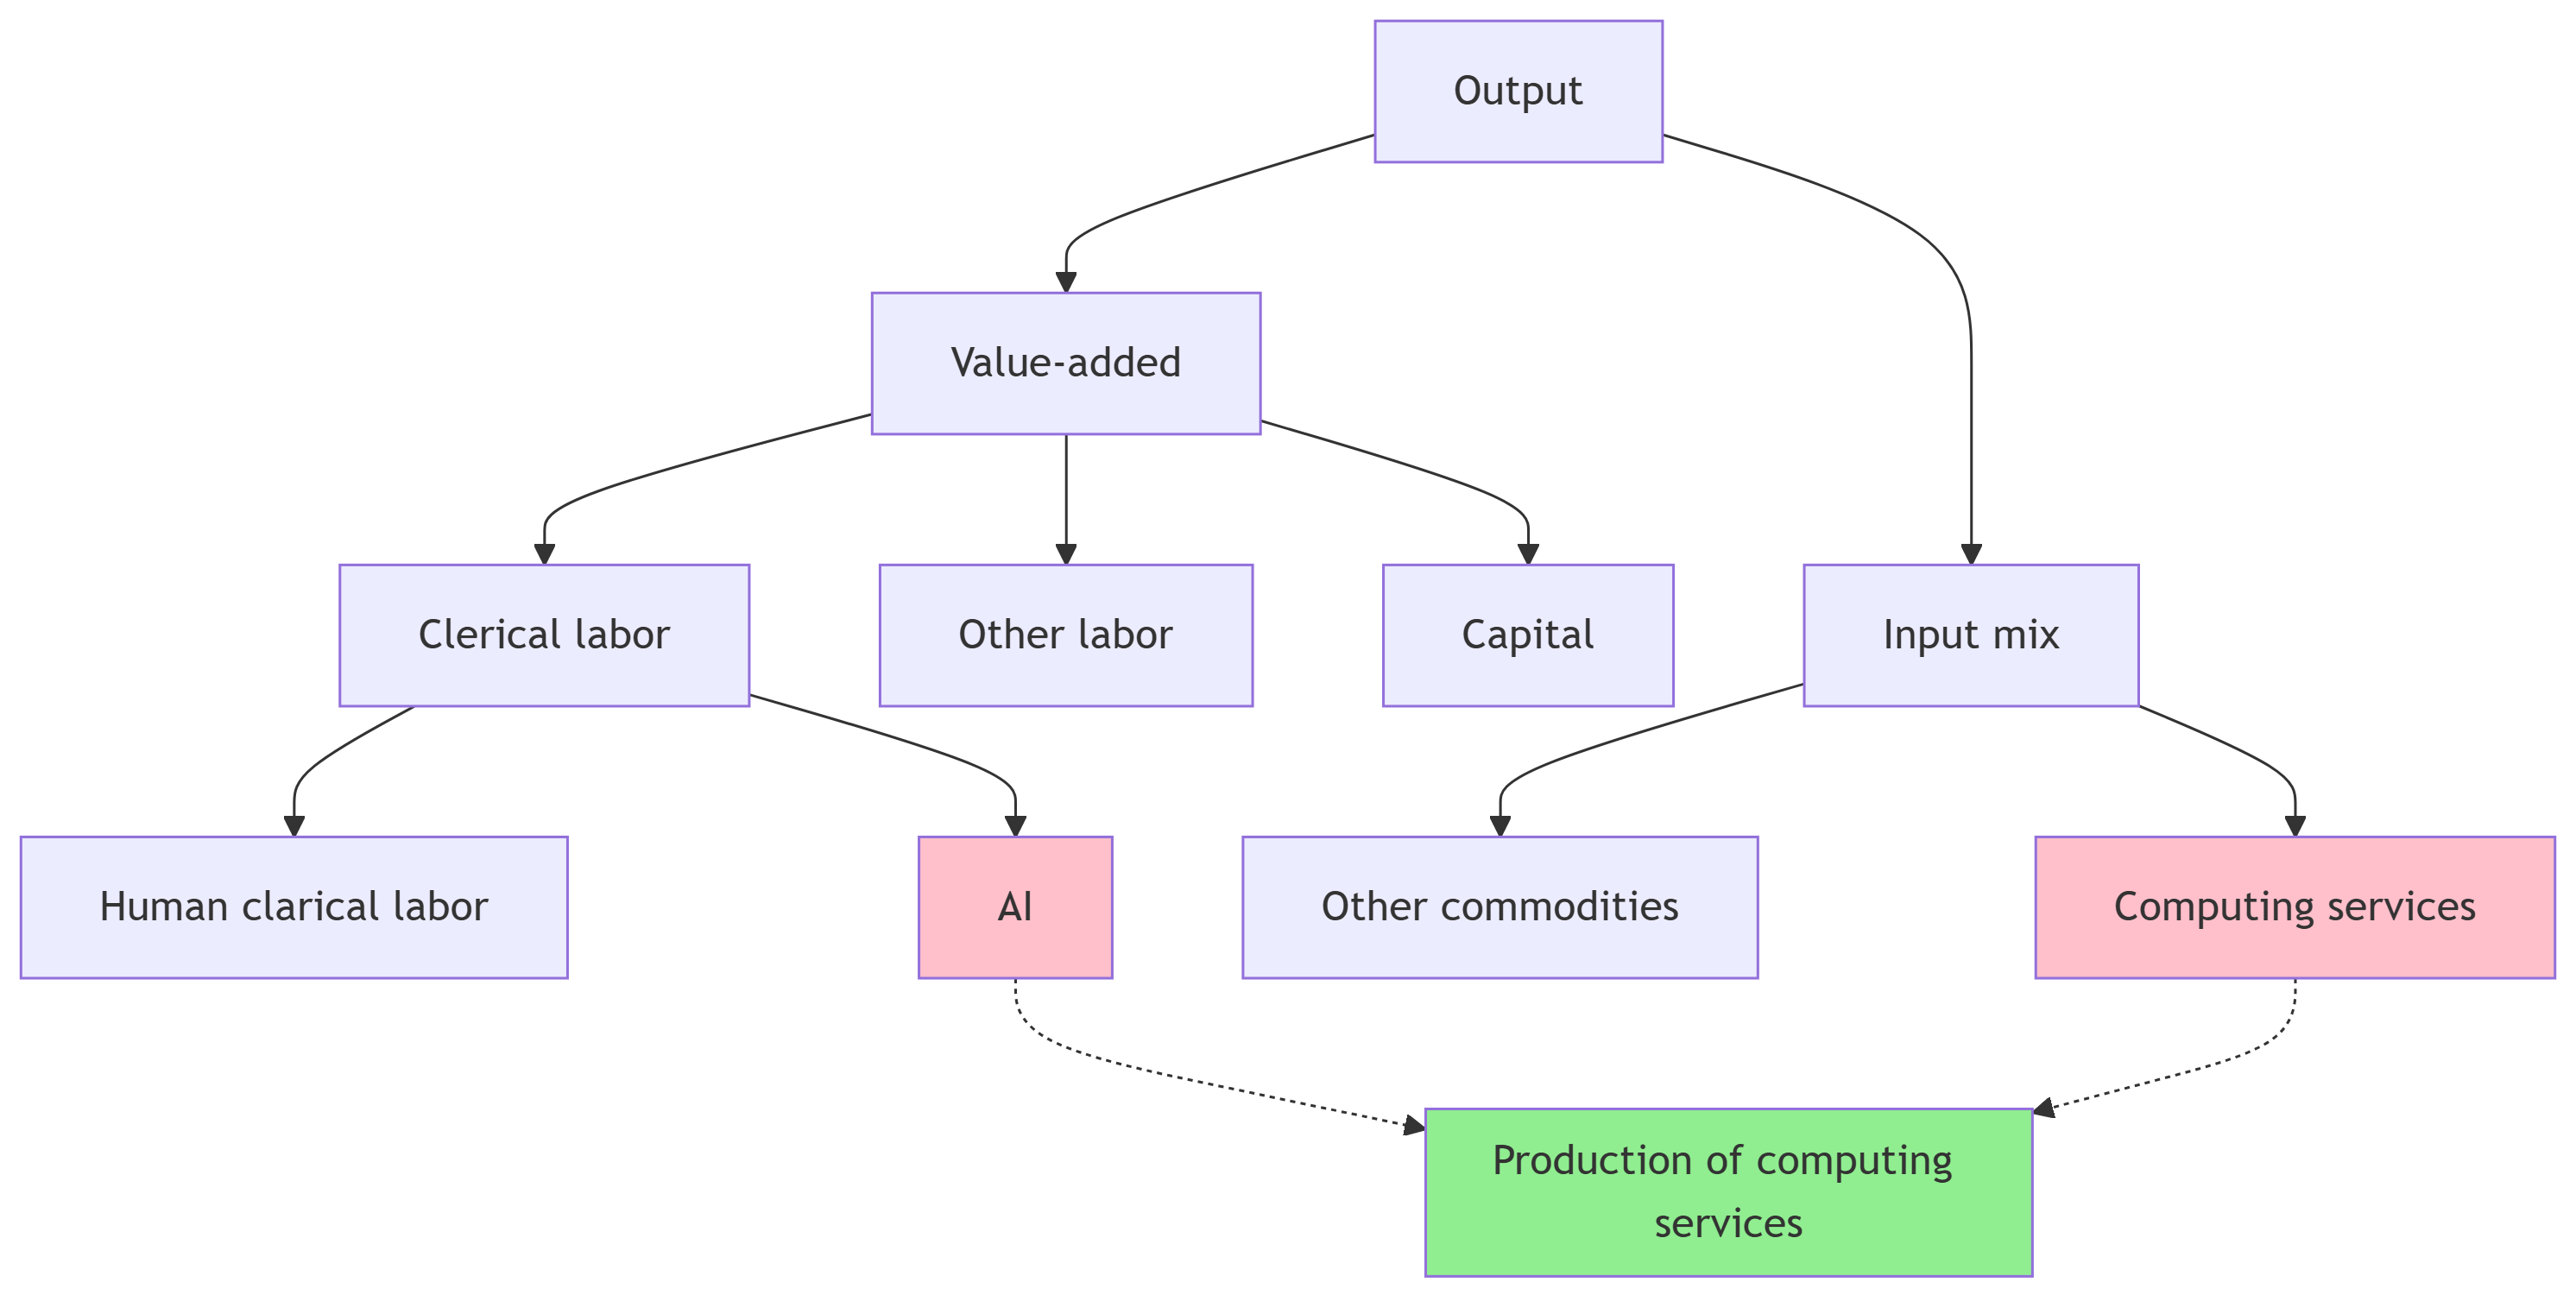
\includegraphics[width=5in,height=2.52in]{mermaid-figure-1.png}

}

\caption{\label{fig-AI-GTAP}Introduction of AI in the production
function (the green nodes show the production of computing service
activity) whose output can be used as either labor-replacing AI or
computing services as an input (in pink)}

\end{figure}%

There are many options to combine AI (\(A\)) and human labor (\(L\)) to
arrive at effective labor \(L_E\) used by industries. If we assume that
AI may be used at various intensities (\(\psi\)) to replace one unit of
human labor, the relation may look like this:

\[L_E = \psi A + L\]

To use this relationship in the GTAP model, we approximate it by a CES
production function:

\begin{equation}\phantomsection\label{eq-labor-combination}{L_E = \gamma \left( \alpha_A A^\rho + \left(1-\alpha_A \right) L^\rho \right)^\frac{1}{\rho}}\end{equation}

where \(\gamma = \frac{\psi+1}{1}\) and
\(\alpha_A = \frac{\psi+1}{\psi}\)

This more flexible functional form allows for a perfect additive
relationship when \(\rho=1\) (perfect substitution). It also allows us
to set \(\rho<1\) to simulate the situation where AI and human labor
cannot replace each other perfectly, requiring both in the production
process. In this work we assume that the substitutability between AI and
human labor is high, with the elasticity of substitution equal to 20
(\(\rho=0.95\)). However, even with this high level of substitution, the
model would never allow for a complete replacement of human labor with
AI or vice versa.

\section{Scenario}\label{scenario}

We are interested in exploring the implications of allowing AI, a
service generated by the information industry, to replace labor at
various costs, for different industries and for different regions.
Specifically, we focus on clerical labor which is the GTAP labor type
that is most likely to be replaced by AI in all industries.\footnote{\citet{manning2026}
  note that clerical and administrative roles are most at risk. They are
  both considered clerical in GTAP.}

We calibrate our model by setting the domestic price of AI and labor to
one in the country with the highest clerical wages (the United States);
we then set the relative wages of clerical labor in other regions to
equal the relative total clerk wages per capita of each country/region.
Furthermore, we assume \(\psi=1\), i.e., one unit of labor can be
substituted by one unit of AI Equation~\ref{eq-labor-combination}. For
the relative wages assumed in the scenarios see Table~\ref{tbl-wages}.

\scriptsize

\begin{longtable}[]{@{}ll@{}}
\caption[Relative per-capita GDPs (assumed to represent relative
clerical wages) ]{Relative per-capita GDPs (assumed to represent
relative clerical wages)\footnote{Source: the GTAP database, version 12}
}\label{tbl-wages}\tabularnewline
\toprule\noalign{}
Region & Wages \\
\midrule\noalign{}
\endfirsthead
\toprule\noalign{}
Region & Wages \\
\midrule\noalign{}
\endhead
\bottomrule\noalign{}
\endlastfoot
Argentina & 0.35 \\
Australia & 0.78 \\
Brazil & 0.14 \\
Canada & 0.75 \\
China & 0.17 \\
EU & 0.29 \\
India & 0.03 \\
Japan & 0.32 \\
Mexico & 0.05 \\
New Zealand & 0.5 \\
ROW & 0.06 \\
Russia & 0.03 \\
South Africa & 0.11 \\
South Korea & 0.6 \\
UK & 0.41 \\
USA & 1.0 \\
\end{longtable}

\normalsize

Much like our building of the model, other AI papers have had to make
similar assumptions. Focusing on \citet{acemoglu2025}, he assumes that
19.9 percent of U.S. labor tasks are exposed to AI, 23 percent of
computer tasks can be profitably performed by AI, and the average labor
cost savings to be 27 percent--which, together, imply an average cost
savings of 15.4 percent. One thing not mentioned in his work is the
potential costs coming from AI, such as energy needs. Given that our AI
sector comes with costs to produce AI (as given in input-output models),
we are able to account for the costs and the benefits of AI.

Because of a wide range of clerical wages across the world and a global
price for tradeable AI, it is likely that adoption of AI may vary across
countries. As we explain earlier, we introduce a different production
function for clerical labor that allows the combination of human labor
and AI. However, changing production is likely to be costly; to account
for this in our model, we assume that if a country or a region's use of
AI falls below a small threshold (1 percent of total labor), then the
country would not adopt AI at all.

We consider two main scenarios in this paper that differ in their
assumptions on the supply of clerical labor: in the ``no unemployment''
scenario, we assume full employment, a standard assumption of the GTAP
model, which results in wage adjustments. In the ``unemployment''
scenario, we assume that nominal wages remains fixed and, instead,
clerical labor exits/enters the labor force to maintain this wage.
Finally, for each scenario we implement a range of taxes on the use of
AI by the industry in the range from 0 to 100 percent.

\section{Data}\label{data}

We use GTAP datbase version 12 with the reference year 2023 aggregated
to 16 regions, seven commodities and seven factors. The regions are:
Australia, New Zealand, China+Hong Kong, Japan, India, Canada, USA,
Mexico, Argentina, Malaysia, South Korea, Brazil, EU, UK, Russia, South
Africa and the rest of the world (ROW) (See Table~\ref{tbl-regions} for
details). The commodities are: crops, animals, extract, food, manuf,
svces and AI (communications and information sector) (See
Table~\ref{tbl-commodities} for details). The factors include all seven
GTAP factors, i.e., land, technical and other professionals
(tech\_aspros), clerks, service staff (service\_shop), officers,
managers and professionals (off\_mgr\_pros), agricultural and other low
skill labor (ag\_othlowsk), capital, and natural resources (natlres).

\scriptsize

\begin{longtable}[]{@{}
  >{\raggedright\arraybackslash}p{(\linewidth - 2\tabcolsep) * \real{0.0940}}
  >{\raggedright\arraybackslash}p{(\linewidth - 2\tabcolsep) * \real{0.9060}}@{}}
\caption{Regional aggregation }\label{tbl-regions}\tabularnewline
\toprule\noalign{}
\begin{minipage}[b]{\linewidth}\raggedright
Region
\end{minipage} & \begin{minipage}[b]{\linewidth}\raggedright
GTAPRegions
\end{minipage} \\
\midrule\noalign{}
\endfirsthead
\toprule\noalign{}
\begin{minipage}[b]{\linewidth}\raggedright
Region
\end{minipage} & \begin{minipage}[b]{\linewidth}\raggedright
GTAPRegions
\end{minipage} \\
\midrule\noalign{}
\endhead
\bottomrule\noalign{}
\endlastfoot
Argentina & arg \\
Australia & aus \\
Brazil & bra \\
Canada & can \\
China & chn, hkg \\
EU & aut, bel, bgr, hrv, cyp, cze, dnk, est, fin, fra, deu, grc, hun,
irl, ita, lva, ltu, lux, mlt, nld, pol, prt, rou, svk, svn, esp, swe \\
India & ind \\
Japan & jpn \\
Mexico & mex \\
New Zealand & nzl \\
ROW & (rest of regions) \\
Russia & rus \\
South Africa & zaf \\
South Korea & kor \\
UK & gbr \\
USA & usa \\
\end{longtable}

\normalsize

\scriptsize

\begin{longtable}[]{@{}
  >{\raggedright\arraybackslash}p{(\linewidth - 2\tabcolsep) * \real{0.1810}}
  >{\raggedright\arraybackslash}p{(\linewidth - 2\tabcolsep) * \real{0.8190}}@{}}
\caption{Commodity aggregation }\label{tbl-commodities}\tabularnewline
\toprule\noalign{}
\begin{minipage}[b]{\linewidth}\raggedright
Aggregate commodity
\end{minipage} & \begin{minipage}[b]{\linewidth}\raggedright
GTAP commodities
\end{minipage} \\
\midrule\noalign{}
\endfirsthead
\toprule\noalign{}
\begin{minipage}[b]{\linewidth}\raggedright
Aggregate commodity
\end{minipage} & \begin{minipage}[b]{\linewidth}\raggedright
GTAP commodities
\end{minipage} \\
\midrule\noalign{}
\endhead
\bottomrule\noalign{}
\endlastfoot
ai & cmn \\
animals & ctl, oap, rmk, wol \\
crops & pdr, wht, gro, v\_f, osd, c\_b, pfb, ocr \\
extract & frs, fsh, coa, oil, gas, oxt \\
food & cmt, omt, vol, mil, pcr, sgr, ofd, b\_t \\
manuf & tex, wap, lea, lum, ppp, p\_c, chm, bph, rpp, nmm, i\_s, nfm,
fmp, ele, eeq, ome, mvh, otn, omf \\
svces & ely, gdt, wtr, cns, trd, afs, otp, wtp, atp, whs, ofi, ins, rsa,
obs, ros, osg, edu, hht, dwe \\
\end{longtable}

\normalsize

\section{Results}\label{results}

\subsection{Who adopts AI and in which
sectors?}\label{who-adopts-ai-and-in-which-sectors}

The adoption rate of AI to replace clerical labor varies across regions
and sectors, and depends heavily on the assumption of full employment.
In both scenarios, we only observe four regions that choose to adopt AI,
with the highest clerical wages---Australia, South Korea, Canada and the
USA (Table~\ref{tbl-adoption}). This reflects the fact that with
globally connected price of AI, which is assumed to equal the cost of
clerical labor in the United States in each region before the
implementation of the scenarios, it makes less sense to use it to
replace much cheaper labor in most other countries. In the case of full
employment, when labor does not exit the labor market but instead the
wage adjusts, the adoption is lower because lower wages make AI less
cost effective. We also note that AI's adoption varies by sector as
well, with agricultural sectors (crops and animals) having the lowest
adoption rates.

As a result of these market forces, we observe the highest adoption
rates in the case of United States in the case of the fixed wages
scenario (Table~\ref{tbl-adoption-un}), where the adoption of AI does
not drive the cost of clerical labor down, resulting in full adoption of
AI in all sectors. Canada has slightly lower initial clerical wages,
their adoption rate is about 96 percent in all sectors except crops
(86\%) and animals (92\%). The adoption rates in Australia are
noticeable lower (78\% in industry, about 50\% in agriculture). Finally,
in the case of South Korea, the adoption rate is only 12\% across all
sectors.

When we assume that AI's adoption does not drive labor out of the labor
market but instead it lowers wages, the adoption rates of AI drop
significantly in all countries that adopt it and in all sectors, as it
becomes less cost effective to displace much cheaper labor
(Table~\ref{tbl-adoption-nu}). The adoption rates remain highest in the
USA where they drop from 100 to 45 percent (industry) and about 20
percent in agriculture. The steepest drop in adoption is observed in
Australia, where the adoption rates drops to 18 percent in industries
and about 6 percent in agriculture.

\begin{table}

\caption{\label{tbl-adoption}Adoption of AI by countries and sectors
(share of total clerical labor-ai expenditure)}

\centering{

\scriptsize

\subcaption{\label{tbl-adoption-nu}No employment assumption}

\centering{

\begin{tabular}{lllll}
\toprule
Commodity & Australia & South Korea & Canada & USA\\
\midrule
crops & 0.06 & 0.06 & 0.1 & 0.19\\
animals & 0.06 & 0.06 & 0.18 & 0.21\\
extract & 0.18 & 0.06 & 0.29 & 0.45\\
food & 0.18 & 0.06 & 0.29 & 0.45\\
manuf & 0.18 & 0.06 & 0.29 & 0.45\\
svces & 0.18 & 0.06 & 0.29 & 0.45\\
ai & 0.18 & 0.06 & 0.29 & 0.45\\
\bottomrule
\end{tabular}

}

\normalsize

\scriptsize

\subcaption{\label{tbl-adoption-un}Unemployment assumption}

\centering{

\begin{tabular}{lllll}
\toprule
Commodity & Australia & South Korea & Canada & USA\\
\midrule
crops & 0.49 & 0.12 & 0.86 & 1.0\\
animals & 0.5 & 0.12 & 0.92 & 1.0\\
extract & 0.78 & 0.12 & 0.96 & 1.0\\
food & 0.78 & 0.12 & 0.96 & 1.0\\
manuf & 0.78 & 0.12 & 0.96 & 1.0\\
svces & 0.78 & 0.12 & 0.96 & 1.0\\
ai & 0.78 & 0.12 & 0.96 & 1.0\\
\bottomrule
\end{tabular}

}

\normalsize

}

\end{table}%

To understand the vast difference between AI adoptions in the two
scenarios, it is important to consider the impact of labor supply
assumption on wages which we show in Table~\ref{tbl-wages-aiprice}. The
decline in clerical wages in the USA is the greatest at -37 percent when
AI is adopted, reducing the demand for clerical labor. The wage decline
is smaller in the rest of the countries that adopt AI, falling by 20
percent in Canada, 14 percent in Australia and 5 percent in South Korea.
Naturally, the strong decline in wages counters AI adoption even though
the price of AI also falls in this scenario albeit at a slower rate,
e.g., the price of AI falls by only 4 percent in the USA.

\scriptsize

\begin{longtable}[]{@{}lll@{}}
\caption{Wage impacts on AI adopting countries with full employment
assumption}\label{tbl-wages-aiprice}\tabularnewline
\toprule\noalign{}
Region & Clerical wages & AI price \\
\midrule\noalign{}
\endfirsthead
\toprule\noalign{}
Region & Clerical wages & AI price \\
\midrule\noalign{}
\endhead
\bottomrule\noalign{}
\endlastfoot
Australia & -14.1 \% & -0.5 \% \\
South Korea & -4.9 \% & -0.2 \% \\
Canada & -19.6 \% & -0.4 \% \\
USA & -36.7 \% & -4.4 \% \\
\end{longtable}

\normalsize

\subsection{Who are the winners and losers of AI
adoption?}\label{who-are-the-winners-and-losers-of-ai-adoption}

Because the impact of replacing clerical labor with AI has economy-wide
impacts, we now consider the changes to other factor owners and we
contrast them to the overall change in consumer prices (shown in
Table~\ref{tbl-marketprices}). The tables show that the impacts on
returns and consumer prices across countries and scenarios are very
mixed. In the full employment scenario, we observe the returns to land
owners to rise substantially in the USA while falling by a similar rate
in Canada. The returns to capital in the USA falls but they increase in
Australia, South Korea and Canada. The impacts on consumer prices are
mixed as well with consumer prices falling in all countries except
Canada. In the fixed wage scenario the impacts are very similar.

Even though the impacts on factor returns and consumer prices are mixed,
the impacts on welfare (EV), are much more consistent. In all countries
except South Korea, we observe an increase in welfare when full
employment is assumed. On the other hand, when labor is allowed to leave
the labor market under fixed wage scenario, the welfare impacts are
unambiguously negative.

\begin{table}

\caption{\label{tbl-marketprices}Impact of the adoption of AI on factor
returns, consumer prices (CPI) and welfare (EV) (percent)}

\centering{

\scriptsize

\subcaption{\label{tbl-marketprices-nu}No unemployment assumption}

\centering{

\begin{tabular}{lllll}
\toprule
Item & Australia & South Korea & Canada & USA\\
\midrule
tech\_aspros & -0.08 & 0.07 & 3.28 & -1.41\\
clerks & -14.09 & -4.88 & -19.6 & -36.75\\
service\_shop & -0.22 & -0.14 & 2.24 & -1.97\\
off\_mgr\_pros & -0.21 & -0.02 & 2.49 & -2.04\\
ag\_othlowsk & -0.0 & -0.07 & 2.27 & 0.83\\
capital & 0.59 & 0.25 & 4.03 & -0.69\\
land & 2.23 & -0.25 & -6.91 & 7.68\\
CPI & -0.69 & -0.15 & 0.08 & -3.84\\
EV & 0.04 & -0.29 & 1.05 & 0.78\\
\bottomrule
\end{tabular}

}

\normalsize

\scriptsize

\subcaption{\label{tbl-marketprices-un}Unemployment assumption}

\centering{

\begin{tabular}{lllll}
\toprule
Item & Australia & South Korea & Canada & USA\\
\midrule
tech\_aspros & -1.65 & 0.31 & 4.24 & -3.35\\
clerks & -0.0 & 0.0 & -0.0 & -0.0\\
service\_shop & -2.12 & -0.13 & 0.78 & -4.81\\
off\_mgr\_pros & -2.1 & 0.13 & 2.11 & -5.09\\
ag\_othlowsk & -1.46 & 0.0 & 2.13 & 0.22\\
capital & 0.68 & 0.71 & 6.36 & -2.35\\
land & 3.82 & -1.85 & -15.33 & 6.52\\
CPI & -0.77 & 0.56 & 0.94 & -4.99\\
EV & -5.7 & -1.7 & -6.79 & -5.08\\
\bottomrule
\end{tabular}

}

\normalsize

}

\end{table}%

\subsection{How does the adoption of AI impact those countries that do
not adopt
AI?}\label{how-does-the-adoption-of-ai-impact-those-countries-that-do-not-adopt-ai}

Having observed that the sign of the welfare change in the countries
that adopt AI to replace clerical labor depends on whether the displaced
labor stays in the market of not, we next consider the implications for
the welfare of the rest of the world shown in
Figure~\ref{fig-welfare-world}. An interesting observation of this
result is that regardless of the scenario selected, i.e., with full
employment or fixed wages, the rest of the countries benefit from the
adoption of AI in the four countries. The benefits in the unemployment
scenario are larger at about 320 billion US dollars than in the full
employment scenario at about 120 billion US dollars. It is also
important to note that even though the adoption of AI is expected to
benefit the countries that do not adopt it, their gain is much smaller
than the impact on the adopting countries. Therefore, the global impact
of AI adoption is driven by what happens in those countries that adopt
it; in the case when displaced labor leaves the labor market the global
welfare falls by about 1.2 trillion US dollars; in the case when
clerical labors stays in the market at a lower wage the world gains a
little over 300 billion US dollars in welfare.

\begin{figure}

\begin{minipage}{0.50\linewidth}

\centering{

\pandocbounded{
\includegraphics[keepaspectratio]{figure-ev-unemployemt.png}}

}

\subcaption{\label{fig-welfare-world-unemployment}Unemployment
assumption}

\end{minipage}%
%
\begin{minipage}{0.50\linewidth}

\centering{

\pandocbounded{
\includegraphics[keepaspectratio]{figure-ev-nounemployemt.png}}

}

\subcaption{\label{fig-welfare-world-nounemployment}No unemployment
assumption}

\end{minipage}%

\caption{\label{fig-welfare-world}Welfare impacts of the adoption of AI
on the adopting countries, the rest of the countries, and the world (in
billions of US dollars)}

\end{figure}%

To see specifically the impact of each country adopting AI to replace
clerical labor on each country's welfare, we perform a decomposition of
the welfare results with respect to each country's
contribution.\footnote{We perform the decomposition by running the
  entire simulation sequentially, adding each country's shocks by sector
  and recording the impact of each additional shock on each country's
  welfare.} We show the results in Figure~\ref{fig-welfare-world-dec}.
Clearly, the vast majority of welfare impacts, whether positive or
negative, are caused by the adoption of AI in the United States. Even
though the impact of the US' own adoption dominates in affecting other
countries' welfare, we note that in the scenario allowing for
unemployment, Australia's, South Korea's and Canada's own negative
impacts dominate their total welfare change. In the case of no
unemployment scenario, however, the positive impact of the US adoption
generally dominates, with the exception fo South Korea whose own impact
drives its overall welfare impact negative.

\begin{figure}

\begin{minipage}{0.50\linewidth}

\centering{

\pandocbounded{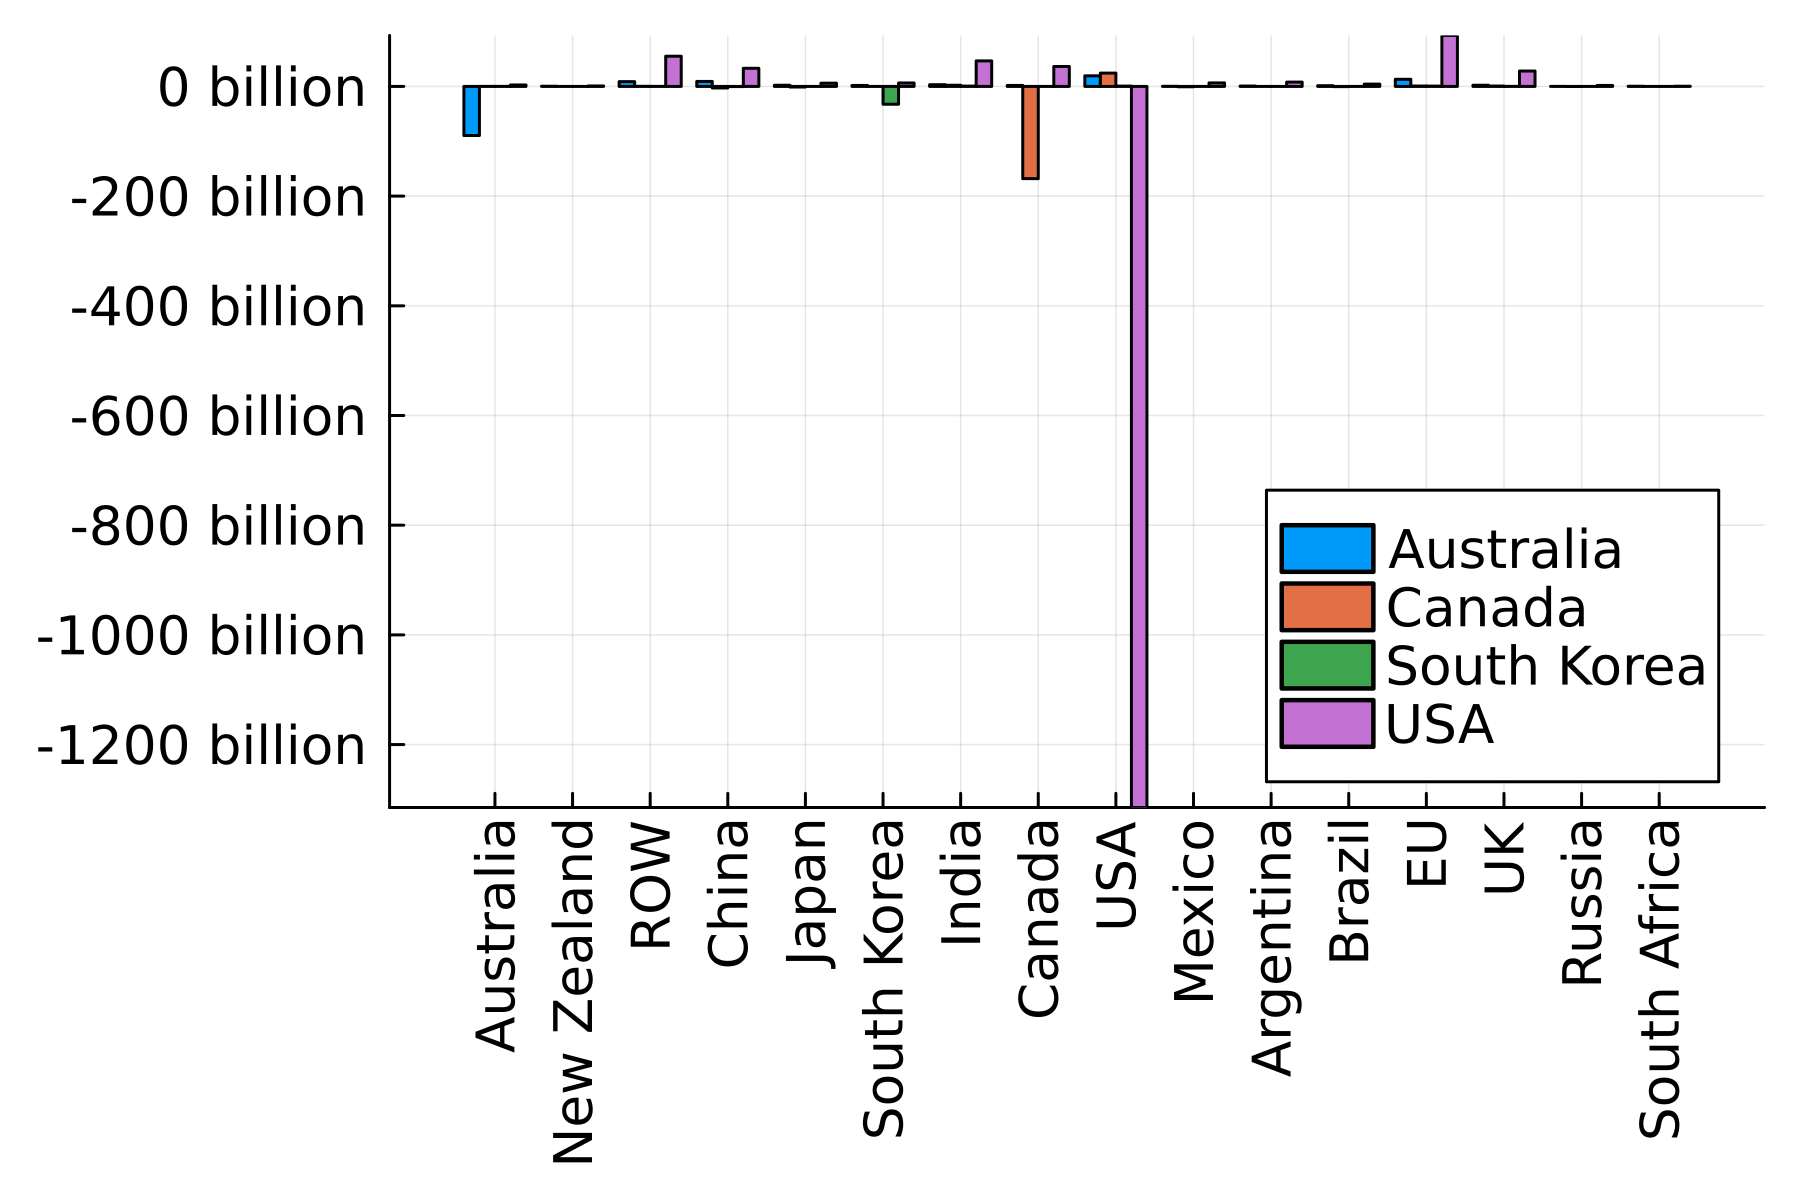
\includegraphics[keepaspectratio]{ev-dec-world_unemployment.png}}

}

\subcaption{\label{fig-welfare-dec-world-unemployment}Unemployment
assumption}

\end{minipage}%
%
\begin{minipage}{0.50\linewidth}

\centering{

\pandocbounded{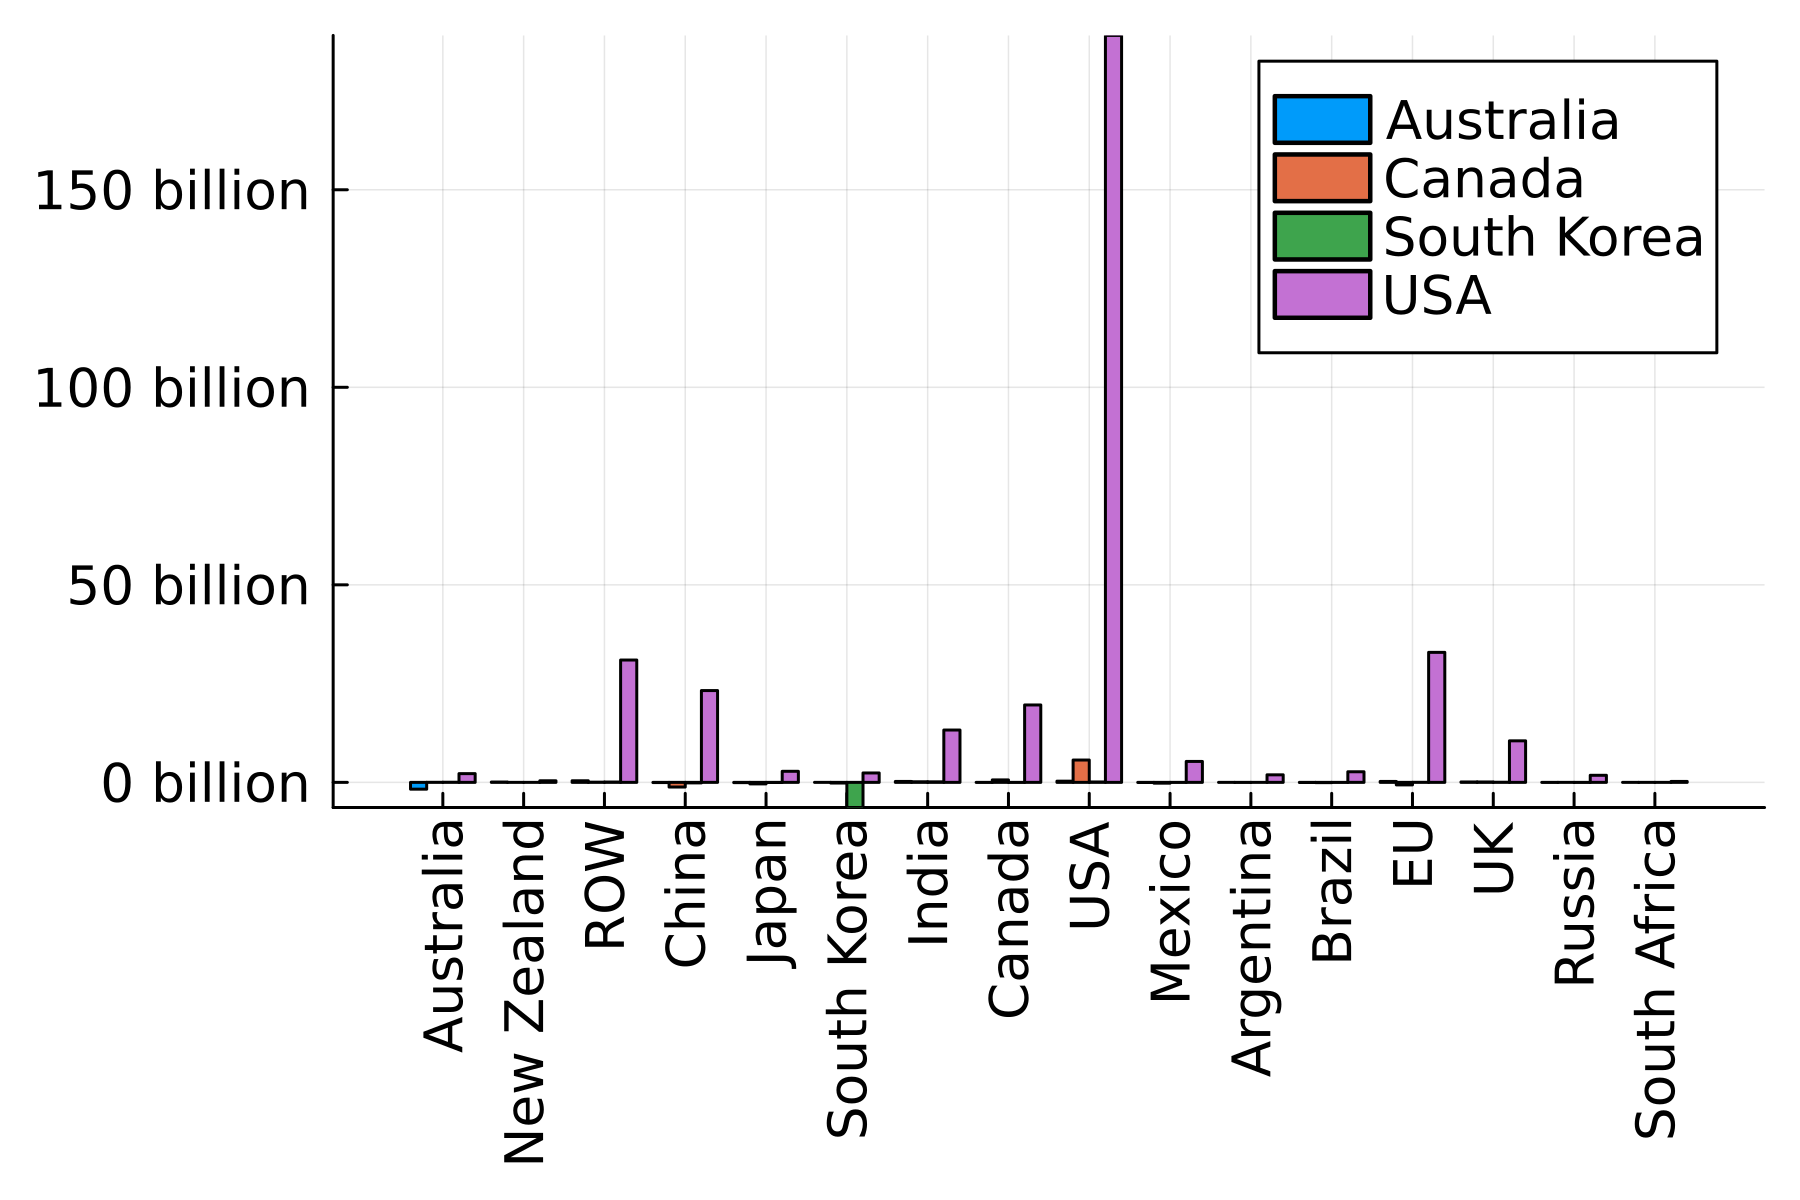
\includegraphics[keepaspectratio]{ev-dec-world_nounemployment.png}}

}

\subcaption{\label{fig-welfare-dec-world-nounemployment}No unemployment
assumption}

\end{minipage}%

\caption{\label{fig-welfare-world-dec}Welfare impacts of the adoption of
AI on the adopting countries, the rest of the countries, and the world
(in billions of US dollars)}

\end{figure}%

\subsection{How does a tax on AI use affect the
adoption?}\label{how-does-a-tax-on-ai-use-affect-the-adoption}

Having described two scenarios of global adoption of AI to replace
clerical labor, we now consider the implication of taxing computing
service when used as a replacement for clerical labor. We consider
several rates of the tax ranging from 0 to 100 percent. In
Figure~\ref{fig-equivalent-variation-tax}, we show the resulting impact
of the tax on global welfare for both assumptions of unemployment (red)
and no unemployment (blue). The figure shows that with a tax rate of
95\% (or higher) all adoption of AI ceases, resulting in no welfare
change to the world. The exact impact of the tax on AI adoption and
welfare depends on the whether the displaced clerical labor stays in the
market (the no-unemployment assumption) or exits the market (the
unemployment assumption). In the former case, increasing the tax rate on
AI from 0 to 100 percent would almost linearly reduce its initial
benefits to the global economy. On the other hand, if clerical labor
exits the labor market, a tax rate below 35 percent would have only a
small impact on the associated welfare loss (associated with AI's
adoption); to prevent a substantial portion of the welfare loss
associated with AI adoption under this assumption, a tax rate of 50\% or
more is required.

\begin{figure}

\centering{

\pandocbounded{
\includegraphics[keepaspectratio]{figure-tax-ev-both.png}}

}

\caption{\label{fig-equivalent-variation-tax}Global EV (billions of USD)
as a result of implementing a technology that allows for replacement of
clerical labor with AI on par for three labor assumptions for various
global AI use tax rates}

\end{figure}%

\clearpage

\section{Conclusion}\label{conclusion}

The Industrial Revolution, the Assembly Line, the mechanization of
agriculture, robots on factory floors---these are all technological
innovations that forced a realignment of labor. In each of these
instances, laborers had to adapt to the situation, whether it was from
learning a new skill or finding a new job. These innovations all led to
leaps in global productivity, shaping the world as we now it today. The
AI transition seems to be the next great technological innovation, one
that will also force a realignment of labor. Unlike those noted
previously, this innovation seems that it will affect higher skilled
more than unskilled labor. But, like all the others, capital is key and
the gains seem like they will accrue to those with the means to procure
the innovation.

Given the potential for AI to affect many aspects of the global economy,
there has been a lot of recent media attention and research. However, it
is clear that it is difficult to forecast labor interactions with, as
well as the understanding potential productivity gains. In our work, we
simulate the case where AI replaces human, clerical labor without
improving productivity of labor. We show with the assumption that AI is
internationally traded (i.e., it has a global price) it is likely that
only the most developed countries with higher initial wages would invest
in AI to replace clerical labor.

We also show that the impact of such an adoption is likely to impact the
welfare of the adopting countries by a large amount; however the sign of
the welfare impact largely depends on the response of the clerical labor
to the new market conditions: if the displaced clerical labor exits the
market, AI adoption would result in an overall welfare loss. However, if
clerical labor stays in the market and accepts lower wages, AI would
boost the supply of labor and, in turn, adopting countries' welfare.

Finally, we consider the implication of taxing computing services when
used in the form of AI to replace labor. We observe that a tax close to
100 percent would be required to make the adoption of AI infeasible.
However, the impact of a smaller tax would depend on the response of the
displaced clerical workers---in the world where clerical workers exit
the labor market, a tax of over 50 percent would be required to make a
substantial impact of reducing the negative welfare implications of AI
adoption.

As mentioned above, there are many aspects of AI that are still unknown,
and can change in the future. By making AI operational within a common
CGE framework, the standard GTAP model, we have built the capacity to
consider additional implications and modalities of AI adoption,
including its adoption in developing countries at a lower cost, or its
interaction with productivity and other policies commonly simulated in
CGE models.

\setcounter{section}{0}
\renewcommand{\thesection}{\Alph{section}}

\setcounter{table}{0}
\renewcommand{\thetable}{A\arabic{table}}

\setcounter{figure}{0}
\renewcommand{\thefigure}{A\arabic{figure}}

\newpage

\section{Appendix}\label{appendix}

\scriptsize

\begin{longtable}[]{@{}
  >{\raggedright\arraybackslash}p{(\linewidth - 6\tabcolsep) * \real{0.2727}}
  >{\raggedright\arraybackslash}p{(\linewidth - 6\tabcolsep) * \real{0.2818}}
  >{\raggedright\arraybackslash}p{(\linewidth - 6\tabcolsep) * \real{0.3000}}
  >{\raggedright\arraybackslash}p{(\linewidth - 6\tabcolsep) * \real{0.1455}}@{}}
\caption{GDP per capita, and agricultural and service labor shares
}\label{tbl-gdp-labor-shares}\tabularnewline
\toprule\noalign{}
\begin{minipage}[b]{\linewidth}\raggedright
Country
\end{minipage} & \begin{minipage}[b]{\linewidth}\raggedright
Share of labor in agriculture
\end{minipage} & \begin{minipage}[b]{\linewidth}\raggedright
Share of labor in manufacturing
\end{minipage} & \begin{minipage}[b]{\linewidth}\raggedright
GDP per capita
\end{minipage} \\
\midrule\noalign{}
\endfirsthead
\toprule\noalign{}
\begin{minipage}[b]{\linewidth}\raggedright
Country
\end{minipage} & \begin{minipage}[b]{\linewidth}\raggedright
Share of labor in agriculture
\end{minipage} & \begin{minipage}[b]{\linewidth}\raggedright
Share of labor in manufacturing
\end{minipage} & \begin{minipage}[b]{\linewidth}\raggedright
GDP per capita
\end{minipage} \\
\midrule\noalign{}
\endhead
\bottomrule\noalign{}
\endlastfoot
Afghanistan & 42.5 & \texttt{missing} & 497 \\
Albania & 36.42 & \texttt{missing} & 6,069 \\
Algeria & 9.6 & \texttt{missing} & 4,468 \\
Angola & 50.73 & 2.55 & 2,494 \\
Argentina & 0.06 & 11.35 & 9,956 \\
Armenia & 24.05 & 9.51 & 4,597 \\
Australia & 2.56 & 7.47 & 55,195 \\
Austria & 3.66 & 15.91 & 49,886 \\
Azerbaijan & 36 & 5.42 & 4,806 \\
Bahamas & 2.2 & 2.81 & 33,640 \\
Bahrain & 0.94 & \texttt{missing} & 27,260 \\
Bangladesh & 38.3 & \texttt{missing} & 2,130 \\
Barbados & 2.65 & 2.79 & 21,912 \\
Belarus & 11.06 & 17.43 & 6,838 \\
Belgium & 0.92 & 12.06 & 46,717 \\
Belize & 16.8 & 7.98 & 6,172 \\
Benin & 38.27 & 13.75 & 1,131 \\
Bhutan & 55.78 & 7.48 & 3,577 \\
Bolivia & 30.54 & 11.22 & 4,203 \\
Bosnia and Herzegovina & 17.96 & 18.64 & 6,122 \\
Botswana & 19.9 & 6.73 & 7,172 \\
Brazil & 9.08 & 11.59 & 9,030 \\
Brunei & 1.95 & 4.3 & 30,427 \\
Bulgaria & 6.62 & 18.56 & 10,354 \\
Burkina Faso & 26.21 & 5.39 & 765 \\
Burundi & 86.21 & \texttt{missing} & 234 \\
Cambodia & 34.53 & 15.09 & 2,226 \\
Cameroon & 43.49 & \texttt{missing} & 1,555 \\
Canada & 1.51 & 9.15 & 46,353 \\
Cape Verde & 10.6 & 9.65 & 4,381 \\
Central African Republic & 69.85 & \texttt{missing} & 449 \\
Chad & 75.06 & \texttt{missing} & 893 \\
Chile & 8.98 & 9.8 & 14,496 \\
China & 25.33 & 28.14 & 10,343 \\
Colombia & 15.77 & 11.66 & 6,473 \\
Comoros & 34.38 & \texttt{missing} & 1,510 \\
Congo & 33.53 & \texttt{missing} & 2,488 \\
Costa Rica & 11.97 & 10.06 & 12,885 \\
Cote d'Ivoire & 40.15 & 6.91 & 2,142 \\
Croatia & 6.19 & 17.81 & 15,564 \\
Cuba & 17.4 & \texttt{missing} & 9,232 \\
Cyprus & 2.41 & 7.27 & 29,227 \\
Czechia & 2.66 & 27.44 & 24,063 \\
Democratic Republic of Congo & 64.3 & \texttt{missing} & 504 \\
Denmark & 2.22 & 10.96 & 59,404 \\
Djibouti & 24.55 & \texttt{missing} & 2,837 \\
Dominican Republic & 8.78 & 10.09 & 8,183 \\
Ecuador & 29.74 & 10.26 & 6,205 \\
Egypt & 20.62 & 12.96 & 2,963 \\
El Salvador & 16.29 & 14.85 & 4,320 \\
Equatorial Guinea & 39.51 & \texttt{missing} & 6,804 \\
Estonia & 3.17 & 18.46 & 24,021 \\
Eswatini & 12.15 & \texttt{missing} & 3,913 \\
Ethiopia & 66.63 & \texttt{missing} & 793 \\
Fiji & 17.61 & \texttt{missing} & 5,842 \\
Finland & 3.78 & 12.93 & 48,358 \\
France & 2.53 & 11.77 & 40,408 \\
French Polynesia & 6.83 & \texttt{missing} & 21,583 \\
Gabon & 29.96 & \texttt{missing} & 7,441 \\
Gambia & 27.03 & \texttt{missing} & 738 \\
Georgia & 38.15 & 5.8 & 4,741 \\
Germany & 1.21 & 18.88 & 47,656 \\
Ghana & 29.75 & \texttt{missing} & 2,187 \\
Greece & 11.6 & 9.62 & 19,335 \\
Guatemala & 31.3 & 11.65 & 4,512 \\
Guinea & 60.65 & \texttt{missing} & 1,031 \\
Guinea-Bissau & 60.48 & 5.55 & 811 \\
Guyana & 15.44 & 10.33 & 6,406 \\
Haiti & 29.03 & \texttt{missing} & 1,352 \\
Honduras & 29.49 & 13.72 & 2,502 \\
Hong Kong & 0.17 & 2.71 & 48,359 \\
Hungary & 4.72 & 22.12 & 17,013 \\
Iceland & 4.04 & 9.34 & 69,296 \\
India & 42.6 & 12.33 & 2,041 \\
Indonesia & 28.5 & 14.38 & 4,107 \\
Iran & 17.37 & 17.56 & 3,997 \\
Iraq & 18.27 & \texttt{missing} & 5,672 \\
Ireland & 4.43 & 10.95 & 81,828 \\
Israel & 0.92 & 9.97 & 44,251 \\
Italy & 3.89 & 18.5 & 33,813 \\
Jamaica & 15.22 & 6.34 & 6,031 \\
Japan & 3.38 & 14.69 & 40,416 \\
Jordan & 2.47 & 8.87 & 4,170 \\
Kazakhstan & 14.86 & \texttt{missing} & 9,457 \\
Kenya & 54.34 & 6.85 & 1,960 \\
Kuwait & 1.78 & \texttt{missing} & 31,708 \\
Kyrgyzstan & 19.32 & 12.09 & 1,422 \\
Laos & 61.44 & \texttt{missing} & 2,589 \\
Latvia & 7.29 & 13.15 & 17,295 \\
Lebanon & 11.32 & 10.85 & 8,906 \\
Lesotho & 44.3 & 22.56 & 1,082 \\
Liberia & 42.62 & \texttt{missing} & 658 \\
Libya & 16.41 & \texttt{missing} & 9,963 \\
Lithuania & 6.44 & 15.88 & 19,609 \\
Luxembourg & 0.68 & 3.46 & 112,697 \\
Macao & 0.4 & 1.62 & 81,883 \\
Madagascar & 64.12 & \texttt{missing} & 500 \\
Malawi & 76.36 & \texttt{missing} & 581 \\
Malaysia & 10.28 & 17.79 & 10,920 \\
Maldives & 8.32 & 9.72 & 11,740 \\
Mali & 62.44 & 5.29 & 972 \\
Malta & 1.02 & 11.06 & 32,422 \\
Mauritania & 30.83 & 6.55 & 1,767 \\
Mauritius & 5.97 & 12.73 & 11,568 \\
Mexico & 12.48 & 16.85 & 10,370 \\
Moldova & 20.96 & 7.1 & 4,405 \\
Mongolia & 25.32 & 7.23 & 4,348 \\
Montenegro & 7.15 & 5.97 & 8,749 \\
Morocco & 33.25 & \texttt{missing} & 3,508 \\
Mozambique & 70.22 & \texttt{missing} & 519 \\
Myanmar & 48.85 & 10.35 & 1,426 \\
Namibia & 21.85 & \texttt{missing} & 4,732 \\
Nepal & 64.38 & \texttt{missing} & 1,203 \\
Netherlands & 2.08 & 8.99 & 53,555 \\
New Caledonia & 1.87 & 2.54 & 33,411 \\
New Zealand & 5.84 & 9.13 & 42,856 \\
Nicaragua & 30.6 & \texttt{missing} & 1,959 \\
Niger & 72.54 & 6.42 & 562 \\
Nigeria & 34.97 & 10.74 & 3,190 \\
North Macedonia & 13.92 & 19.91 & 6,719 \\
Norway & 2.04 & 7.67 & 76,431 \\
Oman & 3.99 & \texttt{missing} & 19,180 \\
Pakistan & 36.92 & 15.08 & 1,390 \\
Panama & 14.41 & 7.54 & 16,478 \\
Papua New Guinea & 56.15 & \texttt{missing} & 2,576 \\
Paraguay & 18.72 & 10.43 & 5,821 \\
Peru & 27.37 & 8.7 & 7,037 \\
Philippines & 22.86 & 8.53 & 3,401 \\
Poland & 9.15 & 20.52 & 15,875 \\
Portugal & 5.5 & 17.03 & 23,343 \\
Qatar & 1.17 & 7.38 & 66,841 \\
Romania & 21.24 & 18.91 & 12,910 \\
Russia & 5.83 & 14.17 & 11,448 \\
Rwanda & 62.29 & 5.38 & 810 \\
Samoa & 30.21 & \texttt{missing} & 4,352 \\
Sao Tome and Principe & 19.14 & \texttt{missing} & 1,935 \\
Saudi Arabia & 2.41 & \texttt{missing} & 29,567 \\
Senegal & 30.1 & 12.86 & 1,431 \\
Serbia & 15.61 & 18.68 & 7,756 \\
Sierra Leone & 54.49 & \texttt{missing} & 844 \\
Singapore & 0.03 & 9.61 & 65,952 \\
Slovakia & 2.79 & 24.61 & 19,406 \\
Slovenia & 4.28 & 25.6 & 25,814 \\
Solomon Islands & 37.26 & \texttt{missing} & 2,224 \\
Somalia & 80.28 & 10.66 & 540 \\
South Africa & 5.28 & 10.77 & 6,534 \\
South Korea & 5.14 & 16.26 & 33,827 \\
Spain & 4.03 & 12.4 & 29,787 \\
Sri Lanka & 24.98 & 18.39 & 4,082 \\
Sudan & 38.37 & \texttt{missing} & 710 \\
Suriname & 8.08 & \texttt{missing} & 6,630 \\
Sweden & 1.69 & 10.01 & 51,649 \\
Switzerland & 2.59 & 12.77 & 84,122 \\
Syria & 10.13 & \texttt{missing} & 1,110 \\
Tajikistan & 44.72 & \texttt{missing} & 871 \\
Tanzania & 65.09 & \texttt{missing} & 1,063 \\
Thailand & 31.43 & 16.28 & 7,606 \\
Togo & 32.38 & 12.8 & 826 \\
Tonga & 19.37 & \texttt{missing} & 4,789 \\
Trinidad and Tobago & 3.03 & 9.08 & 17,213 \\
Tunisia & 13.8 & 18.19 & 3,529 \\
Turkey & 18.11 & 18.35 & 9,395 \\
Turkmenistan & 20.68 & \texttt{missing} & 5,998 \\
Uganda & 72.13 & 3.81 & 822 \\
Ukraine & 13.82 & 13.22 & 3,620 \\
United Arab Emirates & 1.39 & 9.22 & 45,939 \\
United Kingdom & 1.05 & 8.88 & 43,159 \\
United States & 1.36 & 10.42 & 64,746 \\
Uruguay & 8.41 & 10.3 & 18,316 \\
Uzbekistan & 25.71 & 11.91 & 2,041 \\
Vanuatu & 56.78 & 4.02 & 3,207 \\
Venezuela & 7.86 & \texttt{missing} & 2,523 \\
Vietnam & 37.22 & 20.23 & 3,441 \\
Zambia & 49.64 & 4.43 & 1,259 \\
Zimbabwe & 66.19 & 4.41 & 2,184 \\
\end{longtable}

\normalsize

\newpage


\renewcommand\refname{Bibliography}
\begin{thebibliography}{25}
\expandafter\ifx\csname natexlab\endcsname\relax\def\natexlab#1{#1}\fi
\providecommand{\url}[1]{\texttt{#1}}
\providecommand{\href}[2]{#2}
\providecommand{\path}[1]{#1}
\providecommand{\DOIprefix}{doi:}
\providecommand{\ArXivprefix}{arXiv:}
\providecommand{\URLprefix}{URL: }
\providecommand{\Pubmedprefix}{pmid:}
\providecommand{\doi}[1]{\href{http://dx.doi.org/#1}{\path{#1}}}
\providecommand{\Pubmed}[1]{\href{pmid:#1}{\path{#1}}}
\providecommand{\bibinfo}[2]{#2}
\ifx\xfnm\relax \def\xfnm[#1]{\unskip,\space#1}\fi
%Type = Article
\bibitem[{Acemoglu(2025)}]{acemoglu2025}
\bibinfo{author}{Acemoglu, D.}, \bibinfo{year}{2025}.
\newblock \bibinfo{title}{The simple macroeconomics of ai}.
\newblock \bibinfo{journal}{Economic Policy} \bibinfo{volume}{40},
  \bibinfo{pages}{13--58}.
\newblock \URLprefix
  \url{https://academic.oup.com/economicpolicy/article/40/121/13/7728473},
  \DOIprefix\doi{10.1093/epolic/eiae042}.
%Type = Article
\bibitem[{Acemoglu et~al.(2023)Acemoglu, Koster and Ozgen}]{acemoglu}
\bibinfo{author}{Acemoglu, D.}, \bibinfo{author}{Koster, H.},
  \bibinfo{author}{Ozgen, C.}, \bibinfo{year}{2023}.
\newblock \bibinfo{title}{Robots and workers: Evidence from the netherlands} ,
  \bibinfo{pages}{w31009}\URLprefix
  \url{http://www.nber.org/papers/w31009.pdf}, \DOIprefix\doi{10.3386/w31009}.
%Type = Article
\bibitem[{Anderson and Ponnusamy(2023)}]{anderson2023}
\bibinfo{author}{Anderson, K.}, \bibinfo{author}{Ponnusamy, S.},
  \bibinfo{year}{2023}.
\newblock \bibinfo{title}{Structural transformation away from agriculture in
  growing open economies}.
\newblock \bibinfo{journal}{Agricultural Economics} \bibinfo{volume}{54},
  \bibinfo{pages}{62--76}.
\newblock \URLprefix
  \url{https://onlinelibrary.wiley.com/doi/10.1111/agec.12745},
  \DOIprefix\doi{10.1111/agec.12745}.
%Type = Techreport
\bibitem[{Autor and Thompson(2025)}]{autor2025}
\bibinfo{author}{Autor, D.}, \bibinfo{author}{Thompson, N.},
  \bibinfo{year}{2025}.
\newblock \bibinfo{title}{Expertise}.
\newblock \bibinfo{type}{Technical Report}. \bibinfo{address}{Cambridge, MA}.
\newblock \URLprefix \url{http://www.nber.org/papers/w33941.pdf},
  \DOIprefix\doi{10.3386/w33941}.
%Type = Inproceedings
\bibitem[{Bartelings et~al.(2016)Bartelings, Kavallari, Hans and
  Martin}]{bartelings2016}
\bibinfo{author}{Bartelings, H.}, \bibinfo{author}{Kavallari, A.},
  \bibinfo{author}{Hans, v.M.}, \bibinfo{author}{Martin, V.L.},
  \bibinfo{year}{2016}.
\newblock \bibinfo{title}{16th annual conference on global economic analysis},
  \bibinfo{publisher}{GTAP}, \bibinfo{address}{Washington, D.C.}
%Type = Article
\bibitem[{Beckman et~al.(2011)Beckman, Hertel and Tyner}]{beckman2011}
\bibinfo{author}{Beckman, J.}, \bibinfo{author}{Hertel, T.},
  \bibinfo{author}{Tyner, W.}, \bibinfo{year}{2011}.
\newblock \bibinfo{title}{Validating energy-oriented cge models}.
\newblock \bibinfo{journal}{Energy Economics} \bibinfo{volume}{33},
  \bibinfo{pages}{799--806}.
\newblock \URLprefix \url{http://dx.doi.org/10.1016/j.eneco.2011.01.005},
  \DOIprefix\doi{10.1016/j.eneco.2011.01.005}.
%Type = Article
\bibitem[{Beckman et~al.(2021)Beckman, Ivanic and Jelliffe}]{beckman2021}
\bibinfo{author}{Beckman, J.}, \bibinfo{author}{Ivanic, M.},
  \bibinfo{author}{Jelliffe, J.}, \bibinfo{year}{2021}.
\newblock \bibinfo{title}{Market impacts of farm to fork: Reducing agricultural
  input usage}.
\newblock \bibinfo{journal}{Applied Economic Perspectives and Policy}
  \bibinfo{volume}{44}, \bibinfo{pages}{1995--2013}.
\newblock \URLprefix \url{http://dx.doi.org/10.1002/aepp.13176},
  \DOIprefix\doi{10.1002/aepp.13176}.
%Type = Article
\bibitem[{Beckman et~al.(2022)Beckman, Ivanic, Jelliffe and
  Arita}]{beckman2022}
\bibinfo{author}{Beckman, J.}, \bibinfo{author}{Ivanic, M.},
  \bibinfo{author}{Jelliffe, J.}, \bibinfo{author}{Arita, S.},
  \bibinfo{year}{2022}.
\newblock \bibinfo{title}{Adopt or not adopt? mirror clauses and the european
  green deal}.
\newblock \bibinfo{journal}{Applied Economic Perspectives and Policy}
  \bibinfo{volume}{44}, \bibinfo{pages}{2014--2033}.
\newblock \URLprefix
  \url{https://onlinelibrary.wiley.com/doi/10.1002/aepp.13317},
  \DOIprefix\doi{10.1002/aepp.13317}.
%Type = Article
\bibitem[{Beckman et~al.(2023)Beckman, Ivanic and Shaik}]{beckman2023}
\bibinfo{author}{Beckman, J.}, \bibinfo{author}{Ivanic, M.},
  \bibinfo{author}{Shaik, S.}, \bibinfo{year}{2023}.
\newblock \bibinfo{title}{How bilateral trade deals get in the way of
  multilateral agreements: Why wto is marginalized}.
\newblock \bibinfo{journal}{Journal of Policy Modeling} \bibinfo{volume}{45},
  \bibinfo{pages}{877--894}.
\newblock \URLprefix \url{http://dx.doi.org/10.1016/j.jpolmod.2023.05.006},
  \DOIprefix\doi{10.1016/j.jpolmod.2023.05.006}.
%Type = Book
\bibitem[{Clark(1940)}]{clark1940}
\bibinfo{author}{Clark, C.}, \bibinfo{year}{1940}.
\newblock \bibinfo{title}{The Conditions of Economic Progress.}
\newblock \bibinfo{publisher}{Macmillan}.
\newblock \URLprefix
  \url{https://www.jstor.org/stable/10.2307/2225658?origin=crossref},
  \DOIprefix\doi{10.2307/2225658}.
%Type = Article
\bibitem[{Fang et~al.(2024)Fang, Kang and May}]{fang2024}
\bibinfo{author}{Fang, Z.}, \bibinfo{author}{Kang, S.H.}, \bibinfo{author}{May,
  S.M.H.}, \bibinfo{year}{2024}.
\newblock \bibinfo{title}{Does automation really reduce jobs?}
\newblock \bibinfo{journal}{Asia and the Global Economy} \bibinfo{volume}{4},
  \bibinfo{pages}{100099}.
\newblock \URLprefix
  \url{https://linkinghub.elsevier.com/retrieve/pii/S2667111524000239},
  \DOIprefix\doi{10.1016/j.aglobe.2024.100099}.
%Type = Article
\bibitem[{Fisher(1939)}]{fisher1939}
\bibinfo{author}{Fisher, A.}, \bibinfo{year}{1939}.
\newblock \bibinfo{title}{Production: Primary, secondary and tertiary}.
\newblock \bibinfo{journal}{Economics Record} \bibinfo{volume}{15},
  \bibinfo{pages}{24--38}.
%Type = Article
\bibitem[{Gangopadhyay and Mondal(2021)}]{gangopadhyay2021}
\bibinfo{author}{Gangopadhyay, K.}, \bibinfo{author}{Mondal, D.},
  \bibinfo{year}{2021}.
\newblock \bibinfo{title}{Productivity, relative sectoral prices, and total
  factor productivity: Theory and evidence}.
\newblock \bibinfo{journal}{Economic Modelling} \bibinfo{volume}{100},
  \bibinfo{pages}{105509}.
\newblock \URLprefix
  \url{https://linkinghub.elsevier.com/retrieve/pii/S0264999321000985},
  \DOIprefix\doi{10.1016/j.econmod.2021.105509}.
%Type = Techreport
\bibitem[{Hampole et~al.(2025)Hampole, Papanikolaou, Schmidt and
  Seegmiller}]{hampole2025}
\bibinfo{author}{Hampole, M.}, \bibinfo{author}{Papanikolaou, D.},
  \bibinfo{author}{Schmidt, L.D.}, \bibinfo{author}{Seegmiller, B.},
  \bibinfo{year}{2025}.
\newblock \bibinfo{title}{Artificial Intelligence and the Labor Market}.
\newblock \bibinfo{type}{Technical Report}. \bibinfo{address}{Cambridge, MA}.
\newblock \URLprefix \url{http://www.nber.org/papers/w33509.pdf},
  \DOIprefix\doi{10.3386/w33509}.
%Type = Article
\bibitem[{Hertel et~al.(2007)Hertel, Hummels, Ivanic and Keeney}]{hertel2007}
\bibinfo{author}{Hertel, T.}, \bibinfo{author}{Hummels, D.},
  \bibinfo{author}{Ivanic, M.}, \bibinfo{author}{Keeney, R.},
  \bibinfo{year}{2007}.
\newblock \bibinfo{title}{How confident can we be of cge-based assessments of
  free trade agreements?}
\newblock \bibinfo{journal}{Economic Modelling} \bibinfo{volume}{24},
  \bibinfo{pages}{611--635}.
\newblock \URLprefix \url{http://dx.doi.org/10.1016/j.econmod.2006.12.002},
  \DOIprefix\doi{10.1016/j.econmod.2006.12.002}.
%Type = Article
\bibitem[{Hertel et~al.(1997)Hertel, Tsigas et~al.}]{hertel1997structure}
\bibinfo{author}{Hertel, T.W.}, \bibinfo{author}{Tsigas, M.E.}, et~al.,
  \bibinfo{year}{1997}.
\newblock \bibinfo{title}{Structure of gtap}.
\newblock \bibinfo{journal}{Global Trade Analysis: modeling and applications} ,
  \bibinfo{pages}{13--73}.
%Type = Article
\bibitem[{Irwin(2026)}]{irwin}
\bibinfo{author}{Irwin, N.}, \bibinfo{year}{2026}.
\newblock \bibinfo{title}{The ai boom belongs to capital, not workers}.
\newblock \bibinfo{journal}{Axios} \URLprefix
  \url{https://www.axios.com/2026/02/11/ai-boom-labor-market-jobs}.
%Type = Article
\bibitem[{Ivanic(2025)}]{ivanic2025}
\bibinfo{author}{Ivanic, M.}, \bibinfo{year}{2025}.
\newblock \bibinfo{title}{The gtap v7 model in julia}.
\newblock \bibinfo{journal}{Journal of Global Economic Analysis}
  \bibinfo{volume}{10}, \bibinfo{pages}{175--217}.
\newblock \URLprefix \url{http://dx.doi.org/10.21642/JGEA.100104AF},
  \DOIprefix\doi{10.21642/jgea.100104af}.
%Type = Article
\bibitem[{Ivanic et~al.(2023)Ivanic, Beckman and J.~Nava}]{ivanic2023}
\bibinfo{author}{Ivanic, M.}, \bibinfo{author}{Beckman, J.},
  \bibinfo{author}{J.~Nava, N.}, \bibinfo{year}{2023}.
\newblock \bibinfo{title}{Estimation of the value-added/intermediate input
  substitution elasticities consistent with the gtap data}.
\newblock \bibinfo{journal}{Journal of Global Economic Analysis}
  \bibinfo{volume}{8}, \bibinfo{pages}{136--161}.
\newblock \URLprefix \url{http://dx.doi.org/10.21642/JGEA.080204AF},
  \DOIprefix\doi{10.21642/jgea.080204af}.
%Type = Book
\bibitem[{Kuznets(1966)}]{kuznets1966}
\bibinfo{author}{Kuznets, S.}, \bibinfo{year}{1966}.
\newblock \bibinfo{title}{Modern economic growth: Rate, structure and spread}.
\newblock \bibinfo{publisher}{Yale University Press}.
%Type = Techreport
\bibitem[{Manning and Aguirre(2026)}]{manning2026}
\bibinfo{author}{Manning, S.}, \bibinfo{author}{Aguirre, T.},
  \bibinfo{year}{2026}.
\newblock \bibinfo{title}{How Adaptable Are American Workers to AI-Induced Job
  Displacement?}
\newblock \bibinfo{type}{Technical Report}.
\newblock \URLprefix \url{http://dx.doi.org/10.3386/w34705},
  \DOIprefix\doi{10.3386/w34705}.
%Type = Article
\bibitem[{Mills(2025)}]{mills2025}
\bibinfo{author}{Mills, M.}, \bibinfo{year}{2025}.
\newblock \bibinfo{title}{The rise of ai: A reality check on energy and
  economic impacts} .
%Type = Article
\bibitem[{Taheripour et~al.(2010)Taheripour, Hertel, Tyner, Beckman and
  Birur}]{taheripour2010}
\bibinfo{author}{Taheripour, F.}, \bibinfo{author}{Hertel, T.W.},
  \bibinfo{author}{Tyner, W.E.}, \bibinfo{author}{Beckman, J.F.},
  \bibinfo{author}{Birur, D.K.}, \bibinfo{year}{2010}.
\newblock \bibinfo{title}{Biofuels and their by-products: Global economic and
  environmental implications}.
\newblock \bibinfo{journal}{Biomass and Bioenergy} \bibinfo{volume}{34},
  \bibinfo{pages}{278--289}.
\newblock \URLprefix \url{http://dx.doi.org/10.1016/j.biombioe.2009.10.017},
  \DOIprefix\doi{10.1016/j.biombioe.2009.10.017}.
%Type = Article
\bibitem[{UNCTAD(2025)}]{unctad2025}
\bibinfo{author}{UNCTAD}, \bibinfo{year}{2025}.
\newblock \bibinfo{title}{2025 technology and innovation report} .
%Type = Article
\bibitem[{Weinstock and Tierno(2025)}]{weinstock}
\bibinfo{author}{Weinstock, L.}, \bibinfo{author}{Tierno, P.},
  \bibinfo{year}{2025}.
\newblock \bibinfo{title}{The macroeconomic effects of artificial intelligence}
  , \bibinfo{pages}{IF12762}\URLprefix
  \url{https://www.congress.gov/crs-product/IF12762}.

\end{thebibliography}



\end{document}
